%%% Author: Steffen Walter  %%%
%%% Alias: firefly-serenity %%%
%%%%%%%%%%%%%%%%%%%%%%%%%%%%%%%%%%%%%%%%%%%%%%
%%%%%%%%%%%%%%%%%%%%%%%%%%%%%%%%%%%%%%%%%%%%%%
%%% DHBW Stuttgart compliant LaTeX tempalte
%%%%%%%%%%%%%%%%%%%%%%%%%%%%%%%%%%%%%%%%%%%%%%
%%%%%%%%%%%%%%%%%%%%%%%%%%%%%%%%%%%%%%%%%%%%%%

\documentclass[
a4paper,   
titlepage,  
halfparskip,
12pt        
]{scrartcl}  

%%% packages selection for different purposes (see documentation of the package maintainer for more info)
\usepackage[ngerman]{babel}
\usepackage[utf8]{inputenc}
\usepackage[T1]{fontenc}
\usepackage{ae,aecompl}
%\usepackage{helvet}
%\renewcommand{\familydefault}{\sfdefault}
\usepackage{amsmath,amssymb,amstext}
\usepackage{psfrag}
%\usepackage{listings}
%\lstset{language=Python} 
%\usepackage{units}
\usepackage[nottoc]{tocbibind}
\usepackage{cite}
\usepackage{caption}
\usepackage{tabto}
\usepackage{xcolor}
\usepackage{longtable}
\usepackage{lmodern}
\usepackage{setspace}
\usepackage{fancyhdr}
\usepackage{tablefootnote}
\usepackage{acronym}


%%%%%%%%%%%%%%%%%%%%%%%
%%%%%%%%%%%%%%%%%%%%%%%
%%% layout
%%%%%%%%%%%%%%%%%%%%%%%
%%%%%%%%%%%%%%%%%%%%%%%

% Enables blockset
\sloppy

\usepackage{geometry}
\geometry{a4paper, top=25mm, left=30mm, right=25mm, bottom=30mm, headsep=10mm, footskip=12mm}

%%% PDF options

\usepackage{ifpdf}

\ifpdf %if -> pdflatex
  \usepackage[pdftex]{graphicx}

  \pdfcompresslevel=9
  \usepackage[%
    pdftex=true,      
    backref,    
    pagebackref=false,
    colorlinks=false,
    hyperfootnotes=false,
    bookmarks=true,   
    bookmarksopen=false,
    bookmarksnumbered=false, 
    pdfpagemode=None   
  ]{hyperref}
  \DeclareGraphicsExtensions{.pdf}
\else %else -> latex 
  \usepackage[dvips]{graphicx}
  \DeclareGraphicsExtensions{.eps}
  \usepackage[dvips, colorlinks=false]{hyperref}
\fi

%%% PDF-Meta-Information 
\hypersetup{
  pdftitle={T1000},
  pdfauthor={Steffen Walter},
  pdfsubject={Secrets Management in großen Firmenumgebungen},
  pdfcreator={Accomplished with LaTeX2e and pdfLaTeX with hyperref-package.},
  pdfproducer={science + computing ag},
  pdfkeywords={}
}

%%%%%%%%%%%%%%%%%%%%%%%
%%%%%%%%%%%%%%%%%%%%%%%
%%% begin document
%%%%%%%%%%%%%%%%%%%%%%%
%%%%%%%%%%%%%%%%%%%%%%%

%%% header and footer before the actual body

\begin{document}

%%%%%%%%%%%%%%%%%%%%%%%
%%%%%%%%%%%%%%%%%%%%%%%
%%% titlepage
%%%%%%%%%%%%%%%%%%%%%%%
%%%%%%%%%%%%%%%%%%%%%%%

\begin{titlepage}
\begin{longtable}{lcr}
{
\includegraphics[height=1.7cm]{logo}} &
{
\includegraphics[height=1.05cm]{blank}} &
{
\includegraphics[height=1.7cm]{dhbw}}
\end{longtable}
% \enlargethispage{20mm}
\bigskip
\bigskip
\begin{center}
\vspace*{12mm} {\LARGE\bf Secrets Management in großen Firmenumgebungen}\\
\vspace*{12mm} {\large\bf Bericht Praxis I}\\
\vspace*{3mm} {\large\bf T1000}\\
\vspace*{12mm} des Studiengangs Informationstechnik (B.Sc.)\\ an der Dualen Hochschule Baden-Württemberg Stuttgart\\
% \vspace*{3mm} an der Dualen Hochschule Baden-Württemberg\\
\vspace*{12mm} von\\
\vspace*{3mm} {\large\bf Steffen Walter}\\
\vspace*{12mm} 03.09.2018\\
\end{center}
\vfill
\begin{spacing}{1.5}
\begin{tabbing}
mmmmmmmmmmmmmmmmmmmmmmmmmm \= \kill
\textbf{Bearbeitungszeitraum} \> 4 Wochen\\
\textbf{Matrikelnummer, Kurs} \> 1145690, TINF17IN\\
\textbf{Ausbildungsunternehmen} \> science + computing ag, Tübingen\\
\textbf{Betreuer des Ausbildungsunternehmens} \>Dr. Marcus Camen\\
% \textbf{Gutachter der Hochschule} \> Bernd Beutlin\\
\end{tabbing}
\end{spacing}
\end{titlepage}

%%%%%%%%%%%%%%%%%%%%%%%
%%%%%%%%%%%%%%%%%%%%%%%
%%% Erklärung
%%%%%%%%%%%%%%%%%%%%%%%
%%%%%%%%%%%%%%%%%%%%%%%
\thispagestyle{empty}

\begin{table}[h]
\centering
  \begin{tabular}{| l |}
  \hline
  \\
  \textbf{Erklärung} \\
  \\
  Ich versichere hiermit, dass ich meine Studienarbeit mit dem Thema: \\
  ``Secrets Management in großen Firmenumgebungen`` selbstständig verfasst \\
  und keine anderen als die angegebenen Quellen und Hilfsmittel benutzt habe. \\
  \\
  Ich versichere zudem, dass die eingereichte elektronische Fassung mit der gedruckten \\
  Fassung übereinstimmt. \\ \\
  ............................................................\hspace{0.5cm} ......................................\\
  \textit{Ort} \hspace{1cm} \textit{Datum} \hspace{4.2cm} \textit{Unterschrift}\\
  \\
  \hline
  \end{tabular}
\end{table}
\newpage

%%%%%%%%%%%%%%%%%%%%%%%
%%%%%%%%%%%%%%%%%%%%%%%
%%% Abstract
%%%%%%%%%%%%%%%%%%%%%%%
%%%%%%%%%%%%%%%%%%%%%%%
\thispagestyle{empty}

\large{\textbf{Zusammenfassung}}\\
\\
Das Thema Secrets Management wird zunehmend zu einem zentralen Thema in der
elektronischen Datenverarbeitung.  Unter dem Begriff ist im Folgenden vor
allem der Umgang mit geheimen Informationen gemeint.  Geheim sind
Informationen dann, wenn es schädlich ist wenn diese Informationen
Unbefugten zugänglich sind. Beispiele für derartige Informationen sind
Passwörter, geheime Schlüssel oder geheime Dokumente.  In der
Praxisarbeit soll evaluiert werden welche Anforderungen große Unternehmen
an ihr Secrets Management stellen und welche Programme dabei häufig zum
Einsatz kommen.  In einem weiteren Schritt soll festgestellt werden welche
Anforderungen durch jene Programme nicht erfüllt werden.  Im Anschluss
soll eine voll umfängliche Secrets Management Software daraufhin untersucht
werden, in wie fern Unzulänglichkeiten von gängiger Software behoben
werden können.  Es soll auch beleuchtet werden, welche zusätzlichen
Anforderungen Cloud Umgebungen mit sich bringen.  Hierbei zu beachten ist,
welche Vorteile durch alternative Software zu erzielen sind.  Für die
Evaluierung soll eine virtuelle Umgebung erstellt werden, in welcher die
Funktionen getestet werden.
\newpage
\thispagestyle{empty}

\large{\textbf{Abstract}}\\
\\
The topic of secrets management is becoming an uprising matter in digital data processing.
In this report the term of secrets management is mainly used to describe the handling of confidential information.
Information is considered confidential, if it can be used to to harm the owner of the secret in any way.  
Examples for information that meets this criteria would be password, private digital key or simply confidential documents.
In the paper shall be evaluated which requirements enterprises have for their secrets management and which software is currently used to try and fulfill those needs.
Subsequently the gaps between requirements and the functional range of the used Software shall be emphasized.
Furthermore a secrets management software with a modern approach shall be examined to find out whether or not this software is able to fill in the gaps of traditional software.
Also the aspect of cloud environment shall be considered as a factor of importance. 
To achieve this task a virtual environment shall be implemented to test the features of the chosen software.


%%%%%%%%%%%%%%%%%%%%%%%
%%%%%%%%%%%%%%%%%%%%%%%
%%% dictionaries
%%%%%%%%%%%%%%%%%%%%%%%
%%%%%%%%%%%%%%%%%%%%%%%

\pagestyle{fancy}
\fancyhf{} %% remove all previous settings

\newpage
\tableofcontents
\newpage
\pagestyle{fancy}
\fancyhf{} %% clear all previous settings
\fancyhead[R]{\thepage} %% pagenumber in the upper right corner
\fancyhead[L]{VERZEICHNISSE} %% section description in the upper left corner
\pagenumbering{roman}
\section*{Abkürzungsverzeichnis} %%Title for list of acronyms
\addcontentsline{toc}{section}{Abkürzungsverzeichnis}
\begin{acronym}
 \acro{ACL}{Zugriffskontrollliste (engl. Access Control List)}
 \acro{AD}{Active Directory}
 \acro{API}{Schnittstelle zur Anwendungsprogrammierung (engl. Application Programming Interface)}
 \acro{CAE}{Computer Aided Engineering}
 \acro{IT}{Informationstechnik}
 \acro{MIT}{Massachusetts Institute of Technology}
 \acro{OECD}{Organisation für wirtschaftliche Zusammenarbeit und Entwicklung (engl. Organisation for Economic Co-operation and Development)}
 \acro{TLS}{Transportschicht Sicherheit (engl. Transport Layer Security)}
\end{acronym}
\listoffigures
\listoftables
%%%%%%%%%%%%%%%%%%%%%%%
%%%%%%%%%%%%%%%%%%%%%%%
%%% glossary
%%%%%%%%%%%%%%%%%%%%%%%
%%%%%%%%%%%%%%%%%%%%%%%
\newpage

\pagestyle{fancy}
\fancyhf{} %% clear all previous settings
\fancyhead[R]{\thepage} %% pagenumber in the upper right corner
\fancyhead[L]{GLOSSAR} %% section description in the upper left corner

\section*{Glossar} 
\addcontentsline{toc}{section}{Glossar}
\begin{acronym}
	\acro{Authentifizierung:}{der Identitätsnachweis einer Person, Maschine oder eines Dienstes, gegenüber einer weiteren Instanz} 
	\acro{Autorisierung:}{die explizite Freigabe um auf einen geheimen Inhalt zuzugreifen}
	\acro{Cloud-Computing:} {die Verwendung scheinbar  unendlicher IT-Ressourcen,  die bedarfsgerecht und flexibel zur Verfügung gestellt werden können. Clouds können in unterschielichen Formen betrieben werden, so gibt es sogenannte private, public und hybrid-Clouds. Sie unterscheiden sich darin ob die Clouddienste auf eigener Infrastruktur, bei einem Cloudhoster oder gemischt betrieben werden.\cite[S. 3]{cloud}}
	\acro{Computercluter:}{Bei Computerclustern handelt es sich um eine Ansammlung von, meist identischer, Harware, welche zu einer logischen Einheit zusammengefasst wird. Der Cluster wird meist verwendet um komplexe Berechungen zu lösen, die auf einzenen Computern sehr lange dauern würde.}
	\acro{Dienst:}{eine autarke Einheit, welche eine spezifizierte Aufgabe bzw. Funktionalitaet erfuellt und diese ueber keine klar definierte Schnittstelle zur Verfuegung stellt}
	\acro{KeePass Passwort Safe}{ist ein quelloffener Passwortmanager, dazu designed wurde viele Passörter auf sichere Art und Weise zu speichern. Der Zugang zu diesem Passwortsafe wird allein durch ein einziges Masterpasswort gewährt.}
	\acro{Skalierbarkeit:}{beschreibt die Fähigkeit eines Systems zur flexiblen Änderung ihrer Größe. Der Begriff wird meist dann verwendet wenn es um ein Ausweitung des gefragten Systems geht.}
\end{acronym}

\newpage
\pagestyle{fancy}
\fancyhf{} %% clear all previous settings
\fancyhead[R]{\thepage} %% pagenumber in the upper right corner
\fancyhead[L]{\leftmark} %% section description in the upper left corner
\setcounter{table}{0} %% sets tabel counter to 0 to ignore table from frontpage
\begin{onehalfspacing} %% set space between lines to 1.5
\pagestyle{fancy}
\fancyhf{} %% remove all previous settings
%\renewcommand{\headrulewidth}{0pt} %%% activate to remove seperation line between head and main body
\fancyhead[L]{\leftmark} %% section name and number in the upper left corner
\fancyhead[R]{\thepage} %% pagenumber in upper right corner
\pagenumbering{arabic}

%%%%%%%%%%%%%%%%%%%%%%%
%%%%%%%%%%%%%%%%%%%%%%%
%%% begin main document
%%%%%%%%%%%%%%%%%%%%%%%
%%%%%%%%%%%%%%%%%%%%%%%

\section{Einleitung}
\label{sec:einleitung}

\subsection{Gegenstand und Ziele des Praxisberichts}
\label{subsec:ziele}

\subsection{Einführung in das Thema}
\label{subsec:einfuehrung}
Mit der fortschreitenden Digitalisierung nahezu aller Wirtschaftszweige steigt auch die Relevanz für die Absicherung der daraus resultierenden \ac{IT}-Infrastrukturen.
Zusätzlich zu den eigenen Sicherheitsbelangen des Betreibers einer informationstechnischen Umgebung kommen auch noch gesetzliche Regelungen wie das IT-Sicherheitsgesetz zum Tragen. 
Vor allem im Bezug auf eine zunehmende Verlagerung des \ac{IT}-Betriebs hin zum Cloud-Computing und den damit verbundenen Problemen dezentraler Datenhaltung (vor allem bei den public und hybrid Modellen), entstehen häufig unübersichtliche Sicherheitskonzepte. Durch die große Varianz der Szenarien, vor allem auch in Anbetracht unterschiedlicher Sicherheitsniveaus der Daten sind die verwendeten Konzepte der unterschiedlich.\cite[S. 7f]{risiko}\newline
Spionage- und Sabotage-Angriffe werden aus den unterschiedlichsten Motivationen und auch von den Unterschiedlichsten Objekten verübt. So reicht das Spektrum der Angreifer von Kleinkriminellen über Geheimdienste und Terroristen bis hin zur organisierten Kriminalität. Die Aufgabe der \ac{IT}-Sicherheit besteht also darin, die potentiellen Angreifer in ihren Erwägungen zu berücksichtigen und und die Werte und Geheimnisse der Unternehmen zu schützen. Ein zentraler Faktor bei der Entwicklung eines Sicherheitskonzepts auf dieser Grundlage ist es, ein stringentes Konzept zur Kontrolle der Autorisierung einer Person oder eines Dienstes auf unterschiedliche Bereiche in der zu betreuenden Umgebung. Neben der Autorisierung spielt auch die Authentifizierung, denn es muss zu jedem Zeitpunkt sichergestellt werden, dass die Autorisierung auch der richtigen Person oder Anwendung übertragen wurde.\cite[S. 9]{risiko} 
Der Aufwand welcher für \ac{IT}-Sicherheitskonzept betrieben wird bemisst sich meistens am Schaden, der zu erwarten ist, sollten geheime Daten in die Hände Dritter gelangen. Da es kaum verlässliche Daten zur Quantität der Kosten gibt, die durch einen kritischen Sicherheitsvorfall verursacht werden, ist die daran orientierte Bemessung der Sicherheitsvorkehrungen umstritten. Generell gibt es verschiedene Faktoren die bei der qualitativen Kostenabschätzung berücksichtigt werden müssen, so wird im allgemeinen zwischen direkten und indirekten Kosten unterschieden.\cite[S. 12]{kosten}
\subsubsection{Direkte Kosten}
Die direkten Kosten die durch Wirtschaftsspionage entstehen können bemessen sich zu allererste einmal an dem direkten Wert des gestohlenen Eigentums. Dieser Wert lässt sich ermitteln durch den finanziellen Gegenwert, den das Eigentum hat und an den zu erwartenden Gewinneinbußen durch den Verlust (der Exklusivität) des Eigentums. Weiterhin entstehen direkte Kosten durch die das Desaster-Recovery, das heißt durch die Schritte die eingeleitet werden müssen um den Status Quo wieder herzustellen. Zu guter Letzt werden auch noch diejenigen Kosten hinzugezählt, die durch die Prävention einer Wiederholung des Ereignisses entstehen, dazu zählen Prozessänderungen, Sicherheitsunterweisungen und weitere direkte Maßnahmen.\cite[S. 13]{kosten}
\subsubsection{Indirekte Kosten}
Zu den indirekten Kosten werden vor allem die Umsatzausfälle durch Image- und Markenschäden gezählt. Außerdem entstehen hohe Umsatzeinbußen durch Plagiate welche in folge des Gestohlenen Eigentums verbreitet werden können. Plagiate können deutlich günstiger angeboten werden, da die Kosten für Forschung und Entwicklung nicht in den Preis eingerechnet werden müssen.\cite[S. 14]{kosten}
\subsubsection{Versuch einer Quantifizierung}
Nach Schätzungen der \ac{OECD} belaufen sich die Schäden durch Fälschungen und Produktpiraterie weltweit auf 638 Milliarden US-Dollar pro Jahr. Die Schätzungen diesbezüglich gehen aber weit auseinander. Es scheint jedoch Sicher zu sein, dass Sich die Schäden im dreistelligen Milliardenbereich bewegen. Für die deutsche Wirtschaft liegen die Schätzungen zwischen 20 und 50 Milliarden Euro.\cite[S. 16f]{kosten}
\subsubsection{Anforderung an Sicherheitssoftware}
\label{subsubsec:anforderung}
Spezifische Anforderungen die an eine Software zum Secrets Management gestellt werden, können wie folgt zusammengefasst werden:

\begin{itemize}
  \item Auffindbarkeit - Es muss zu jedem Zeitpunkt klar sein, wo sich Secrets im Unternehmen befinden.
  \item Nachvollziehbarkeit - Es muss möglich sein, Verantwortliche zu nennen.
  \item Break Glass Szenario - Es muss einen Weg geben, im Fall eines Angriffs den Schaden einzugrenzen.
  \item Verfügbarkeit - Daten müssen jederzeit zugänglich sein.
  \item Integrität - Daten müssen immer vollständig und korrekt sein.
  \item Verlässlichkeit - Daten müssen authentisch sein, Kommunikationswege nachvollziehbar.
  \item Autorisierung - Der Zugriff auf Daten soll nur dann möglich sein, wenn die betroffene Person/Maschine berechtigt ist (minimale Berechtigungsvergabe).
  \item Benutzerfreundlichkeit - Einfacher Zugriff von Mensch und Maschine.
  \item Authentifizierung - Sichere Anmeldeverfahren müssen zur Verfügung stehen.
  \item Credential Management Systeme zur sicheren Erstellung, Speicherung und Änderung sollen zur Verfügung stehen.
  \item Das Risiko, dass kompromittierte Verschlüsselung zum Verlust oder dem unberechtigten Offenlegen von Informationen führt, muss kontrollierbar sein.
\end{itemize}

Rechtliche Aspekte werden durch den Vorliegenden Bericht nicht weiter beleuchtet.\footnote{Die Inhalte aus \autoref{subsubsec:anforderung} wurden in Anlehnung an interne Dokumenten eines großen Unternehmens und Gesprächen mit \ac{IT}-Administratoren erarbeitet}

\section{Stand der Technik}
\label{subsec:stand}
Um die in \autoref{subsec:einfuehrung} beschriebenen Themenkomplexe der Autorisierung und Authentifizierung in Firmenumgebungen umzusetzen gibt es verschiedene Ansätze. Im folgenden sollen einige gängige Softwareprodukte, die die genannten Aufgaben erfüllen sollen vorgestellt und auf ihre Tauglichkeit zur voll umfänglichen Erfüllung der in \autoref{subsubsec:anforderung} beschriebenen Anforderung untersucht.
\begin{table}[h]
\centering
  \begin{tabular}{|l|c|c|c|}
  \hline
  \textbf{Funktion} & \textbf{Kerberos} & \textbf{Pleasant Pass-} & \textbf{Hashicorp}\\
  Näheres: & & \textbf{word Server} & \textbf{Vault} \\
  \autoref{subsubsec:anforderung} & & (Multi-User KeePass) &\\
  \hline
  \hline
  Auffindbarkeit & \checkmark & \checkmark & \checkmark\\
  \hline
  Nachvollziebarkeit & $\times$ & \checkmark & \checkmark\\
  \hline  
  Break Glass Szenario & $\times$ & $\times$ & \checkmark\\
  \hline
  Verfügbarkeit & \checkmark & \checkmark & \checkmark\\
  \hline
  Integrität & \checkmark & \checkmark & \checkmark\\
  \hline
  Verlässlichkeit & \checkmark & ? & \checkmark\\
  \hline
  Autorisierung & $\times$ & \checkmark & \checkmark\\
  \hline
  Authentifizierung & \checkmark & \checkmark & \checkmark\\
  \hline
  Credential Management & \checkmark & \checkmark & \checkmark\\
  \hline
  Kontrollierbarkeit & $\times$ & \checkmark & \checkmark\\
  \hline
  \end{tabular}
\caption[Softwarevergleich]{Vergleich verschiedener Softwareprodukte\cite[S. 4f, 13, 57 ]{kerberos}\cite{pleasant}\cite{vault}}
\label{tab:ver}
\end{table}
Die Programme werden in unterschiedlichen Versionen angeboten. Einige der beschriebenen Funktionen stehen möglicherweise in der kostenfreien Version nicht zur Verfügung.

\subsection{Kerberos}
Der Name Kerberos kommt ursprünglich aus der griechischen Mythologie, wo er für den dreiköpfigen Hund verwendet wurde, der den Eingang zu Unterwelt bewacht. 
Das Projekt wurde in den achtziger Jahren am \ac{MIT} ins als Teil des sogenannten Athena-Projekts ins Leben gerufen. Die großen Stärken von Kerberos liegen in der Authentifizierung und der verschlüsselten Nachrichtenübermittlung. Schon zu Beginn des Projekts lag, neben den Sicherheitsaspekten, der Fokus ganz klar auf der Skalierbarkeit des Systems. 
Verschlüsselt wird mit symmetrischer Verschlüsselung und einem vorher vereinbarten geheimen Schlüssel. Kerberos unterstützt inzwischen auch den Einsatz von Passwörtern, ist dafür aber ursprünglich nicht entwickelt worden. 
Mit diesen Grundfunktionen kann eine relative sichere und authentisierte Kommunikation zwischen Nutzer und Dienst in einem Umfangreichen Netzwerk gewährleistet werden.\newline
Durch die Tatsachen, dass die Software unter einer Open-Source-Lizenz veröffentlicht wurde, können Sicherheitslücken schnell aufgespürt und behoben werden. Außerdem ist es dadurch möglich, dass Unterschildleiche Unternehmen an dem Code mitarbeiten und diesen ständig verbessern und dies geschieht auch zum Beispiel durch Microsoft. Kerberos kommt heutzutage selten als Einzelsystem vor, sondern es wird entweder mit anderen Softwarekomponenten kombiniert, oder es kommt als Bestandteil einer umfangreicheren Software wie zum Beispiel Microsoft \ac{AD} vor.\cite[S. 137f]{kerberos2}\newline
Die Authentifizierung mit Kerberos wird über sogenannte Tickets organisiert. Der Client fordert ein Ticket beim Authentifizierungsserver an. Der Authentifizierungsserver verschlüsselt anschließend das Ticket mit dem Schlüssel des Clients und dem Schlüssel des gewünschten Dienstes. Mit diesem Ticket kann der Client sich nun mit dem gewünschten Dienst verbinden und es ist gewährleistet, dass sowohl der Dienst, als auch der Client diejenigen sind für die sie sich ausgeben.  Der Zugrundeliegende Ablauf wird in \autoref{fig:kerb} nochmal genauer und anschaulicher gezeigt. Bei der gegenseitigen Authentifizierung ist es nicht entscheidend auf welchem Betriebssystem Client und Server basieren, weil dies der Fall ist kann bei Kerberos von einer plattformübergreifenden Software gesprochen werden.
\begin{figure}[h]
	\centering
	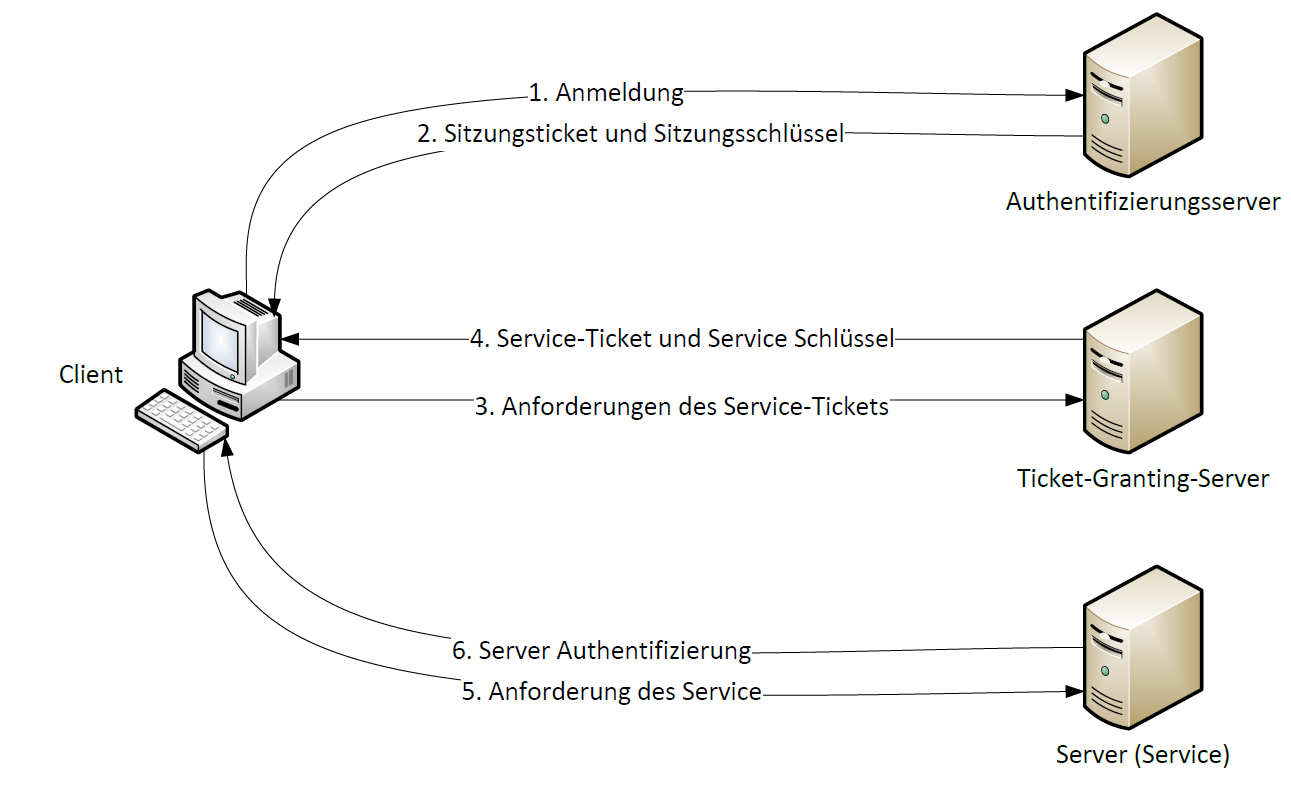
\includegraphics[width=1\linewidth]{kerberos.png}
	\caption[Kerberos]{Authentifizierung mit Kerberberos \cite[vgl. S.140]{kerberos2}}
	\label{fig:kerb}
\end{figure}
Kritisch im Zusammenhang mit Kerberos ist die Fokussierung auf einen Zentralen Server, dieser muss so dimensioniert sein, dass er alle Anfragen verarbeiten kann und, dass durch einen Hardwaredefekt der Betrieb nicht stoppt. Ein weiterer Nachteil ist die fehlende Verschlüsselung des Netzwerkverkehrs. Außerdem werden Sitzungsschlüssel zwischenzeitlich auf dem Client gespeichert und sind so ein leichtes Ziel für Angreifer die Zugriff auf die Clientmaschine haben. Es kann ebenfalls kritisiert werden, dass die Änderung eines Nutzerpassworts immer mit der Änderung des geheimen Schlüssels einhergeht. Im allgemeinen macht Kerberos aber genau das was es soll und seine Popularität zeigt auch, dass es diese Aufgabe sehr zufriedenstellend löst. Mit diversen Erweiterungen lassen sich die erwähnten Unzulänglichkeiten auch umgehen.\cite[vgl. S.138f]{kerberos2}

\subsection{Pleasant Password Server}
Beim Pleasant Password Server Handelt es sich nach eigenen Angaben um eine serverbasierte KeePass Passwort Safe. Im Unterschied zu seinem kleinen Bruder ist der Pleasant Passowrd Server allerdings, wie der Name schon vermuten lässt, keine reine Client Software mehr, sondern er fügt sich als Serverdienst in eine \ac{IT}-Umgebung ein. Das Ziel der Anwendung ist es eine sichere Ablagemöglichkeit für Passwörter, Produkt-Keys, Kreditkarteninformationen und Dateien zu bieten. Zur verschlüsselten Netzwerkkommunikation werden \ac{TLS}-Zertifikate verwendet. Die Client-Software wird als installierbares Programm zur Verfügung gestellt welches auf einigen gängigen Betriebssystemen installiert werden während die Serveranwendung nur für Microsoft Windows zur Verfügung gestellt wird. Es gibt auch einen Webanwendung die eine clientseitig plattformunabhängige Nutzung ermöglicht. 
Eine Rollen- und Eintragsbasierte Rechtevergabe ist vorgesehen, womit der Zugriff durch ausschließlich autorisierte Entitäten sichergestellt werden soll. Mit seiner Initialen Veröffentlichung im Oktober 2012 handelt es sich beim Pleasant Password Server noch um eine relativ junge Software, die jedoch durch den Hersteller, dem Versionsstand nach zu urteilen, regelmäßig mit Updates versorgt wird.\cite{pleasant}
Wie aus \autoref{tab:ver} hervorgeht, erfüllt die Software schon relativ viele der festgelegten Kriterien. Da es sich jedoch nicht um ein quelloffenes Programm handelt, gibt es wenige Informationen über die internen Mechanismen und deren Sicherheit. Aus dem Lizenzmodell geht zudem hervor, dass sich die Software eher an kleine bis mittelständige Unternehmen richtet und somit an der Anforderung eine Lösung für ein Großunternehmen zu bieten vorbei geht.

\subsection{Das Passwort Dilemma}
\label{subsec:pass}
Das Passwort ist die einfachste und am häufigsten verwendete Methode um eine Authentifizierung zwischen einem Mensch und einem Computersystem durchzuführen. Es ist leicht zu implementieren und leicht zu bedienen. Es gibt allerdings eine Reihe an Angriffsszenarien bei denen das klassische Passwort als authentifizierender Faktor versagt.
\begin{itemize}
	\item Das Passwort kann beim Eintippen durch einen dritten gesehen oder gefilmt werden. 
	\item Passwörter können über sogenannte Brute-force Angriffe ``erraten`` werden. Um diese Angriffe durchzuführen gibt es spezielle Programme, die so lange alle möglichen Kombinationen an Tastaturzeichen ausprobieren, bis sie das Passwort herausgefunden haben. 
	\item Wenn Passwörter über das ein Netzwerk übertragen werden, können sie durch spezielle Software abgegriffen werden. Außerdem gibt es spezielle Software, welche die Tastatureingaben am Computer protkollieren kann. Solche Software kann dazu verwendet werden Passwörter die an betreffenden Endgeräten eingegeben werden an einen Angreifer zu übermitteln.
	Ein weiteres Angriffsszenario stellt das sogenannte Login Spoofing dar. Hierbei wird ein Anmeldefenster gefälscht, welches möglichst gleich aussieht wie das original. Wenn der Nutzer sein Passwort in das gefälschte Fenter eingibt, wird es gespeichert oder direkt an den Angreifer übermittelt. 
\end{itemize}
Jeder dieser Angriffe reicht aus um Systeme zu täuschen die zur Authentifizierung allein auf Passwörter setzen. In den meisten Unternehmen ist es aus diesen Gründen nicht erlaubt das gleiche Passwort für unterschiedliche Dienste zu verwenden. Außerdem gibt es versuche durch Passwortrichtlinien die Komplexität der Passwörter zu steigern, sodass zum Beispiel Brute-force Angriffe länger dauern und sich nicht mehr lohnen. Zusätzlich werden Schwellwerte für fehlgeschlagene Anmeldeversuche festgelegt um zu vermeiden, dass Passörter beliebig oft ausprobiert werden können. Diese Maßnahmen verringern zwar die Zahl der erfolgreichen Angriffe, stehen jedoch im Widerspruch zur einfachen Benutzbarkeit. Ein hoher Aufwand für die \ac{IT}-Abteilungen muss aufgebracht werden um Passwörter zurückzusetzen und die Sicherheitsmechanismen für jeden Dienst zu implementieren.\cite[S. 3ff]{hong}
Auf Grund der vielen Angriffsmöglichkeiten gibt es viele Stimmen, die das Ende des Passworts, wie wir es kennen, fordern. Es gibt außerdem viele Empfehlungen ein Passwort am besten zu erzeugen ist um eine Steigerung der Sicherheit gegenüber Angriffen zu erreichen. Was bleibt ist die menschliche Komponente beim Umgang mit Passwörtern. Da Menschen sich auf Bequemlichkeit nicht an die Empfehlungen zur Erstellung eines ``sicheren`` Passworts halten und dies sich auch nur bedingt überprüfen lässt ohne neue Angriffsflächen zu bieten, bleibt das Problem bestehen, dass Passwörter ``geknackt`` werden und Angreifer Zugriff auf sensible Daten bekommen. Es gibt mittlerweile einen Trend zur sogenannten Zwei-Faktor Authentifizierung wobei die zum Identitätsnachweis nicht allein das Passwort verwendet wird, sondern ein weiterer Faktor hinzugenommen wird. Es gibt unterschiedliche Methoden wie solch ein weiterer Faktor aussehen kann, so gibt es zum Beispiel Codes die über die Mobiltelefone der User zugeschickt werden und die nur einmal und für eine kurze Zeitperiode verwendet werden können. Da es bis jetzt aber noch keine vollkommene Alternative zu Passwörtern gibt, ist es sehr wahrscheinlich, dass das Passwort noch einige Zeit also Teil der Authentifizierung bestehen bleiben wird.\cite{pass}
\subsection{Hashicorp Vault}

Bei Vault handelt es sich dem Hersteller Hashicorp zufolge um ein vollumfängliches Secrets Management System. Die Software wird in der Community Edition unter einer Quelloffenen Lizenz veröffentlicht und verfügt über eine umfangreiche Dokumentation. Folgende Funktionen und Funktionsweisen liefert Vault dem Hersteller zufolge:

\textbf{Funktionen von Vault:}
\begin{itemize}
  \item Willkürliche Verbindungen von Identifikator und Wert können auf ``sichere`` Art und Weise durch Vault abgelegt werden. Dabei werden die Inhalte verschlüsselt bevor sie in einen persistenten Speicher geschrieben werden.
  \item Für eine zunehmende Anzahl an Diensten kann Vault dynamische Zugangsdaten generieren. Wenn zum Beispiel ein Dienst Zugriff auf eine Datenbank erhalten will, kann Vault einen (zeitlich Beschränkten) Zugriff gewähren. Dabei werden temporäre Zugangsdaten (oder ein Schlüsselpaar) erstellt, welche durch Vault nach Ablauf der Gültigkeit widerrufen werden.
  \item Daten welche sensible Inhalte haben, können durch Vault verschlüsselt werden, ohne dass sie durch Vault im eigenen Backend gespeichert werden müssen. Entwickler sind damit in der Lage Daten durch Vault verschlüsseln zu lassen um im Anschluss nach Belieben weiterzuverarbeiten.
  \item Alle Geheimnisse welche durch Vault gespeichert werden haben eine Gültigkeitsdauer. Nach Ablauf der zugeordneten Gültigkeitsdauer werden die betroffenen Geheimnisse durch Vault widerrufen. Clients können durch entsprechende Schnittstellen zu Anwendungsprogrammierung (API) die Gültigkeit eines Geheimnisses verlängern bzw. erneuern.
  \item Geheimnisse können auch durch Administratoren widerrufen werden. Dabei bietet Vault die Funktion, dass bei Bedarf ganze Baumstrukturen an Geheimnissen auf einmal ihre Gültigkeit verlieren. Es kann auf unterschiedliche Weisen gefiltert werden, so können zum Beispiel alle Geheimnisse widerrufen werden auf die ein spezieller User zugegriffen hat.
\end{itemize}
\textbf{Die Komponenten von Vault:}
\begin{itemize}
  \item Storage Backend: Vault benötigt ein Storage Backend um verschlüsselte Daten abzulegen. Die einzige Anforderung an das Storage Backend ist, dass es möglichst strapazieren ist. Vault vertraut dem Storage Backend nicht und es wird nicht davon ausgegangen, dass es speziell gegen fremde Zugriffe geschützt ist. 
  \item Barriere: Zwischen Storage und Vault wird jede Kommunikation durch eine Art Kontrollpunkt geprüft. Durch diesen Mechanismus soll sichergestellt werden, dass alle Daten welche von Vault in Richtung Storage Backend übermittelt werden, zwangsläufig verschlüsselt werden. Außerdem ist der Mechanismus dafür zuständig alle Daten die aus dem Storage Backend gelesen werden zu verifizieren und zu entschlüsseln. 
  \item Secrets Speicher: Das Secrets Speicher ist dafür Zuständig auf Anfrage ein angefordertes Geheimnis preiszugeben. Bei einigen Systemen ist der Prozess statisch organisiert. Das bedeutet, dass bei der gleichen Anfrage immer die gleiche Rückgabe zu erwarten ist. Andere Systeme arbeiten hier etwas komplexer, sie sind dazu in der Lage dynamische Zugangsdaten zu erzeugen. Diese Möglichkeit schafft eine zusätzliche Sicherheitsebene. Das Feature steht allerdings nicht für jede Anwendung zur Verfügung
  \item Client Token: Ein Client Token wird ausgestellt, um einen Client über die Dauer einer Sitzung gegenüber Vault zu authentisieren.
  \item Server: Vault wird als einzelne Binärdatei zur Verfügung gestellt, es kann sowohl als Client als auch als Server ausgeführt werden. Wenn der Server gestartet wurde, kümmert er sich um die Kommunikation mit Hintergrunddiensten und stellt ein \acs{API} für die Clientinteraktion bereit. Außerdem ist er verantwortlich für die Anwendung der \ac{ACL}s und den Widerruf abgelaufener Geheimnisse. Neben einigen weiteren Aufgaben erstellt der Server auch ein Log in welchem jede Interaktion mit Vault dokumentiert wird. 
\end{itemize}\cite{vault}

\subsection{Motivation}
In den vorigen Abschnitten wurden Problematiken und Widersprüche aufgezeigt, die zur Wahl des Themas für die vorliegende Arbeit geführt haben. Der Diskurs um Sicherheits- und Secrets- Management in großen Firmenumgebungen (mehrere Niederlassungen) und der Trend hin zur Auslagerung eigener Rechenzentren zu Cloud-Providern, wirft immer wieder die Frage nach funktionierenden Sicherheitskonzepten auf. Nicht zu Letzt, die zunehmenden erfolgreichen Angriffe, die auf ein unzureichendes Sicherheitskonzept zurückzuführen sind werfen die Frage nach einem Umfangreichen Sicherheitssystem auf, welches dazu in der Lage ist neue Bedrohungen und sich verändernde Bedingungen abzudecken. 
Eine der wichtigsten Herausforderungen bei Cloudumgebungen stellt nicht allein das Management von User Zugangsdaten dar es wird immer wichtiger auch die Verwaltung von Diensten und deren Zugangsdaten zu beleuchten. Klassischerweise geht es dabei um Datenbankpasswörter, es kommen aber immmer mehr sogenannte Microservices dazu. Bei Mirsoservices handelt es sich um kleine Programme, die meist eine einzige Aufgabe erfüllen und über eine \ac{API} steuerbar sind. Wenn im Netzwerk viele Microservices aktiv sind, die nicht unwahrscheinlich auch untereinander kommunizieren und sich Authentifizieren müssen, verliert ein Administrator leicht die Übersicht. Auf Grund der Problematiken die in \autoref{subsec:pass} aufgezeigt wurden ist es also essentiell auch hier für einen möglichst sicheren Ablauf zu sorgen um zu erreichen, dass es für Angreifer sehr schwer wird gefälschte Dienste einzuschleusen um an geheime Informationen zu kommen, bzw. bestehende Dienst dafür zu verwenden.\footnote{Eigene Darstellung zur Basis der vorangegangen Abschnitte}

\subsection{Projektumgebung}
Das Thema Sicherheit in der Datenverarbeitung ist seit der Einführung eben jener ein wichtiges Thema. Über die Jahre haben sich die Möglichkeiten zur Absicherung in der \ac{IT} stetig weiterentwickelt, sodass die Absicherung von Computern, Netzwerken, Servern und ganz allgemein Informationen zu einem wichtigen Zweig der Branche geworden ist. Mit neuen Technologien stellt sich immer auch die Frage nach den Sicherheitsaspekten.\newline
Cloud-Computing ist aktuell ein sehr wichtiger und schnell wachsendes Faktor in der \ac{IT}-Branche, vor allem im Ausland werden Technologien rund um das Thema Cloud stark gefördert und es gibt eine Vielzahl an Softwareprodukten die sich diesem Feld verpflichtet haben. Für die Nutzung der Vorteile dieser Technologien in Deutschland gibt es einige Faktoren die es zu betrachten gilt. Zum Beispiel gilt es zu kalkulieren, ob eine Verlagerung von Anwendungen oder Daten auf Cloud Infrastruktur wirtschaftlich ist oder nicht. Dabei spielt die vorhandene Infrastruktur eine Zentrale Rolle und es gilt zu betrachten ob ein schrittweiser oder teilweiser Umzug das Mittel der Wahl sein könnte. Vor diesem Hintergrund spielt natürlich wieder das Thema Sicherheit eine wichtige Rolle. Daten auf ``fremder`` Hardware zu speichern, wie es in Cloud Umgebungen gängige Praxis ist, stellt immer ein Risiko dar. In diesem Kontext muss als immer darauf geachtet werden, dass kritische Daten und Anwendungen nur autorisierten Personen und Anwendungen zur Verfügung gestellt werden. Weiterhin ist abzuwägen in wie fern sich die aktuelle Software, welche zur Authentifizierung und Autorisierung eingesetzt wird, dazu eignet die genannten Herausforderungen zu lösen. In dieser Arbeit soll dieser Aspekt genauer beleuchtet werden.
\subsubsection{Unternehmensvorstellung}
Die science + computing ag, kurz s+c, ist als Tochergesellschaft der ATOS SE ein Unternehmen des \ac{IT}-Dienstleistungs- und Consultingbereichs. Mit seinen knapp 300 Mitarbeitern betätigt sich die s+c hauptsächlich in den Bereichen High Performance Computing, \ac{IT}-Sicherheit, 3D-Virtualisierung und System-Management. Durch OpenSoftware-Dienstleistungen und diverse Softwareprodukte betätigt sich das Unternehmen zudem im Bereich der Softwareentwicklung. Neben Großkunden der Automobilindustrie besteht der diverse Kundenkreis der s+c aus Mikroelektronikherstellern, Chemie- und Pharmaunternehmen, Maschinen- und Anlagenbauer, Forschungs- und Bildungseinrichtungen und Unternehmen aus der Luft- und Raumfahrtbrache. Zum Hauptsitz in Tübingen kommen noch vier weitere Standorte in Berlin, Düsseldorf, Ingolstadt und München hinzu. Bis zur Übernahme durch den französischen Computerhersteller Bull war die 1989 gegründete science + computing ag ein eigenständiges Unternehmen.\cite{bull} Im Jahr 2014 wurde die BULL-Gruppe ihrerseits durch die ATOS SE übernommen wodurch auch die science + computing ag nun zum ATOS-Gesamtkonzern gehört.\cite{atos} ATOS SE ist ein International agierender Konzern mit knapp 100.000 Mitarbeitern, einem jährlichen Umsatz von 14 Milliarden Dollar und Hauptsitz in Bezons (Frankreich). Nach der Forbes Liste der 2000 größten Unternehmen der Welt belegt ATOS SE mit den oben genannten Werten den Platz 858 (Stand Juni 2018).\cite{forbes} Im Zuge der Übernahme durch ATOS SE wird die Marke s+c seit 2016 nicht mehr weitergeführt. Stattdessen wird nun die Konzernmarke ATOS verwendet.

\subsubsection{Arbeitsumgebung}
Die Durchführung der Projektarbeit findet im Team \ac{CAE}3 der science + computing ag statt. Im Team \ac{CAE}3 werden Kunden betreut, die unter Verwendung von High Perfomance Computing Berechnungen anstellen. Der Fokus des Teams liegt dabei auf Kundenkreisen die sich im Bereich \ac{CAE} betätigen. Im Team gibt es verschiedene Kompetenzen um die volle Bandbreite der Kundenwünsche abdecken zu können. Zu den Kernkompetenzen gehören hierbei Weiter-/Entwicklung von systemunterstützender Software, Administration von Computerclustern inklusive Überwachung der Systemkomponenten sowie Administration und Bereitstellung von speziellen Speicherinfrastrukturen. Die Evaluierung welche Teil dieses Praxisberichts ist, soll erste Informationen liefern aus denen sich die Nutzbarkeit von Secrets Management Software zur interne Nutzung ableiten lässt. Der praktische Teil der Evaluierung wird auf einer virtualisierten Umgebung auf Basis von VMware Workstation durchgeführt.

\subsubsection{Unternehmensspezifische Anforderungen}



\section{Hauptteil}
\label{sec:hauptteil}

Teil 1
Theoretische Ausarbeitung als Vorarbeit zur Durchführung
des Projekts

Teil 2
Anforderungsdefinition
Anforderungsanalyse
Lösungsgenerierung
Lösungsbewertung
Umsetzung

\section{Zusammenfassung und Ausblick}
\label{sec:ausblick}


%%%%%%%%%%%%%%%%%%%%%%%
%%%%%%%%%%%%%%%%%%%%%%%
%%% end main document
%%%%%%%%%%%%%%%%%%%%%%%
%%%%%%%%%%%%%%%%%%%%%%%

\appendix
\bibliographystyle{plain}
\bibliography{literatur}

\end{onehalfspacing}
\end{document}

%%%%%%%%%%%%%%%%%%%%%%%%%%%%%%%%%%%%%%%%%%%%%%
%%%%%%%%%%%%%%%%%%%%%%%%%%%%%%%%%%%%%%%%%%%%%%
%%%%%%%%%%%%%%%%%%%%%%%%%%%%%%%%%%%%%%%%%%%%%%
%%%%%%%%%%%%%%%%%%%%%%%%%%%%%%%%%%%%%%%%%%%%%%

